% Section 4: Algorithms
\section{Algorithms}




\subsection{ADMM method for dual problem}
For convenience, introducing relaxation variables, we reformulate the dual problem as:

\begin{equation}
  \begin{array}{rl}
    {\mathrm{(dual)}} & {\min -_{u,v} \sum_{i=1}^{m} \mu_{i} u_{i}-\sum_{j=1}^{n} \nu_{j} v_{j}} + I_{\mathbb{R}_+^{m\times n}}(\xi)\\
    {\text { subject to }} & {c_{ij} - u_i - v_j -\xi_{ij}= 0\qquad\forall i=1, \ldots, m \quad j = 1,\cdots,n}
    \end{array}
\end{equation}

Then we have the augmented Lagrangian:

\begin{equation}
  \begin{aligned}L(u, v, \xi, w)=&-\sum_{i=1}^{m} \mu_{i} u_{i}-\sum_{j=1}^{n} \nu_{j} v_{j} + I_{\mathbb{R}_+^{m\times n}}(\xi)\\&+\sum_{i=1}^{m} \sum_{j=1}^{n} w_{i j}\left(c_{i j}-u_{i}-v_{j}-\xi_{i j}\right)+\frac{\rho}{2} \sum_{i=1}^{m} \sum_{j=1}^{n}\left(c_{i j}-u_{i}-v_{j}-\xi_{i j}\right)^{2}\end{aligned}
\end{equation}

$\partial_{\xi_{ij}} L = 0$ gives:

\begin{equation}
  \xi_{ij} = (c_{ij} - u_i - v_j + \frac{w_{ij}}{\rho})_+
\end{equation}

$\partial_{u_i}L = 0$ gives:

\begin{equation}
  u_i = \frac{1}{n}\left(\frac{\mu_{i}+\sum_{j=1}^{n} w_{i j}}{\rho}+\sum_{j=1}^{n}\left(c_{i j}-v_{j}-\xi_{i j}\right)\right)
\end{equation}

$\partial_{v_j} L = 0$ gives:
\begin{equation}
  v_j = \frac{1}{n}\left(\frac{\nu_{j}+\sum_{i=1}^{m} w_{i j}}{\rho}+\sum_{i=1}^{m}\left(c_{i j}-u_{j}-\xi_{i j}\right)\right)
\end{equation}

\vspace{2ex}
    \begin{algorithm}[htbp]
        \SetAlgoNoLine
        \caption{ADMM method for dual problem} 
        \KwIn{parameters $\mu$, $\nu$, $c$}
        \KwIn{step size $\alpha$, penalty $\rho$}
        Initialize variables $u, v = \boldsymbol{0}$\\
        Initialize variables $\xi, w = \boldsymbol{0}$\\
        \While{ stopping criterion not met } 
        {  
            Update $u$: $\boldsymbol{u} \leftarrow \operatorname{argmin}_{u} L(u, v, \xi, w)$\\
            Update $\pi^{\dagger}$: $\boldsymbol{\pi}^{\dagger} \leftarrow \operatorname{argmin}_{u} L(u, v, \xi, w)$\\
            Update $\xi$: $\boldsymbol{\xi} \leftarrow \operatorname{argmin}_{\xi} L(u, v, \xi, w)$\\
            Update $w$: $\boldsymbol{w} \leftarrow w + \rho\cdot \alpha (\pi - \pi^{\dagger})$\\
        }
    \end{algorithm}

\subsection{Entropic Regularization Methods}
The Kullback-Leibler divergence is defined as 

\begin{equation}
  \mathbf{K L}(\mathbf{P} | \mathbf{Q}) \stackrel{\text { def. }}{=} \sum_{i, j} \mathbf{P}_{i, j} \log \left(\frac{\mathbf{P}_{i, j}}{\mathbf{Q}_{i, j}}\right)-\mathbf{P}_{i, j}+\mathbf{Q}_{i, j}
\end{equation}

with the convention $0 \log(0) = 0$ and $\mathbf{K L}(\mathbf{P} | \mathbf{Q}) = +\infty$ if there exists some $(i, j)$ such that $\mathbf{Q}_{i,j} = 0$ but $\mathbf{P}_{i,j} \neq 0$. The special case $\mathbf{K L}(\mathbf{P} | \mathbf{1})$ corresponds to minus the Shannon-Boltzmann entropy. The function $\mathbf{K L}(\cdot | \mathbf{Q})$ is strongly convex, because its hessian is $\partial^{2} \mathbf{K L}(\mathbf{P} | \mathbf{Q})=\operatorname{diag}\left(1 / \mathbf{P}_{i, j}\right)$ and $\mathbf{P}_{i,j} \leq 1$.

The idea of the entropic regularization of optimal transport is to use $\mathbf{KL}$ as a regularizing function to obtain approximate solutions to the original transport problem:

\begin{equation}
  \label{eq:entropy_regularization}
  \mathrm{L}_{\mathbf{C}}^{\varepsilon}(\mathbf{\mu}, \mathbf{\nu}) \stackrel{\text { def. }}{=} \min _{\mathbf{P} \in \mathbf{U}(\mathbf{\mu}, \mathbf{\nu})}\langle\mathbf{P}, \mathbf{C}\rangle+\varepsilon \mathbf{K L}(\mathbf{P} | \mathbf{\mu} \otimes \mathbf{\nu})
\end{equation}

Here we used as a reference measure for the relative entropy $\mathbf{\mu} \otimes \mathbf{\nu}=\left(\mathbf{\mu}_{i} \mathbf{\nu}_{j}\right)_{i, j}$. This choice of normalization, specially in this discrete setting, has no importance for the selection of the optimal $\mathbf{P}$ since it only affects the objective by a constant, indeed for $\mathbf{P} \in \mathbf{U}(\mathbf{\mu}, \mathbf{\nu})$, one has 

\begin{equation}
  \mathbf{K L}(\mathbf{P} | \mathbf{\mu} \otimes \mathbf{\nu})=\mathbf{K} \mathbf{L}\left(\mathbf{P} | \mathbf{\mu}^{\prime} \otimes \mathbf{\nu}^{\prime}\right)+\mathbf{K} \mathbf{L}\left(\mathbf{\mu}^{\prime} \otimes \mathbf{\nu}^{\prime} | \mathbf{\mu} \otimes \mathbf{\nu}\right)
\end{equation}

At this time, the approximate optimal transport problem has the $\epsilon$-strongly convex objective function, so it has a unique solution. Theoretically, As $\epsilon$ approaches 0, the optimal solution of the approximate optimal transport problem $\mathbf{P}_{\epsilon}$ converges to the optimal solution of the Kantorovich optimal transport problem. At this time, we can use the Sinkhorn algorithm to solve this problem with entropy regularization.

\begin{figure}[htbp]
  \centering
  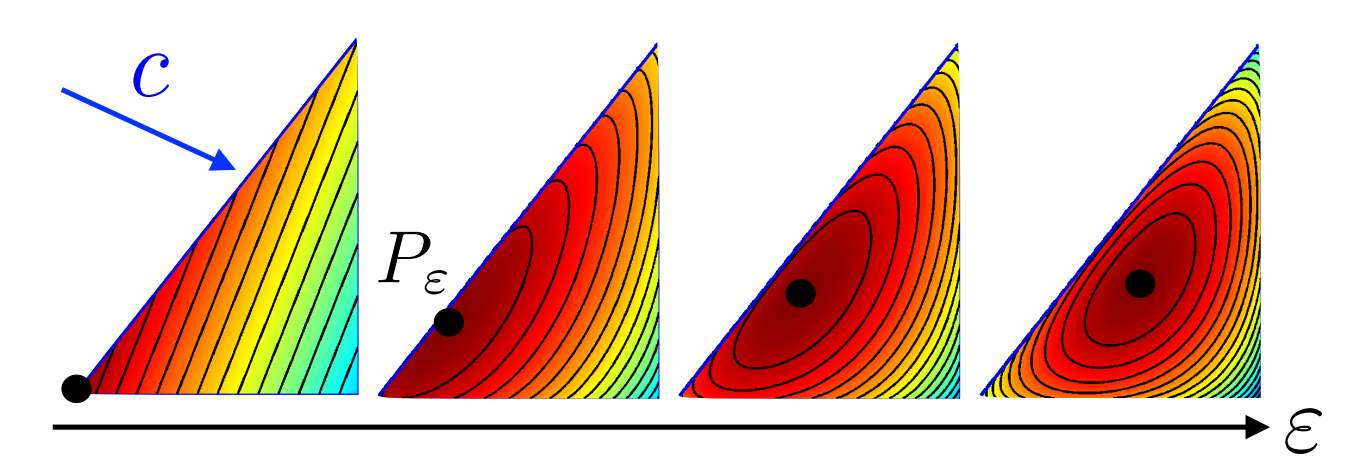
\includegraphics[width=0.9\linewidth]{img/regularized}
  \label{fig:regularized}
  \caption{Impact of $\epsilon$ on the optimization of a linear function on the simplex}
\end{figure}

\subsection{Sinkhorn Algorithm}
The following theorem [4] shows that the solution of \ref{eq:entropy_regularization} has a specific form, which can be parameterized
using $m + n$ variables. That parameterization is therefore essentially dual, in the sense that a coupling $\mathbf{P}$ in
$\mathbf{U}(a, b)$ has $nm$ variables but $n + m$ constraints.

\paragraph{Theorem}
  $\mathbf{P}$ is the unique solution to \ref{eq:entropy_regularization} if and only if there exists $(u, v) \in R$ such that
  
  \begin{equation}
    \label{eq:thm1}
    \forall(i, j) \in [m] \times [n], \quad \mathbf{P}_{i, j}=\mathbf{u}_{i} \mathbf{K}_{i, j} \mathbf{v}_{j}
  \end{equation}
  and $\mathbf{P} \in \mathcal{U}(\mathbf{\mu}, \mathbf{\nu})$.

This can be proved by introducing two dual variables $\mathbf{f} \in \mathbb{R}^{m}, \mathbf{g} \in \mathbb{R}^{n}$ for each marginal constraint, the Lagrangian of \ref{eq:entropy_regularization}
reads

\begin{equation}
  \mathcal{E}(\mathbf{P}, \mathbf{f}, \mathbf{g})=\langle\mathbf{P}, \mathbf{C}\rangle+\varepsilon \mathbf{K} \mathbf{L}(\mathbf{P} | \mathbf{\mu} \otimes \mathbf{\nu})+\left\langle\mathbf{f}, \mathbf{\mu}-\mathbf{P} \mathbf{1}_{m}\right\rangle+\left\langle\mathbf{g}, \mathbf{\nu}-\mathbf{P}^{\mathrm{T}} \mathbf{1}_{n}\right\rangle
\end{equation}

Considering first order conditions (where we ignore the positivity constraint, which can be made rigorous by
showing the associated multiplier vanishes), we have

\begin{equation}
  \label{eq:partial}
  \frac{\partial \mathcal{E}(\mathbf{P}, \mathbf{f}, \mathbf{g})}{\partial \mathbf{P}_{i, j}}=\mathbf{C}_{i, j}+\varepsilon \log \left(\frac{\mathbf{P}_{i, j}}{\mathbf{\mu}_{i} \mathbf{\nu}_{j}}\right)-\mathbf{f}_{i}-\mathbf{g}_{j}=0
\end{equation}

which results, for an optimal $\mathbf{P}$ coupling to the regularized problem, in the expression $\mathbf{P}_{i, j}=\mathbf{\mu}_{i} \mathbf{\nu}_{j} e^{\frac{\mathbf{f}_{i}+\mathbf{g}_{j}-\mathbf{C}_{i, j}}{\varepsilon}}$ 
which can be rewritten in the form provided in the proposition using non-negative vectors
\begin{equation}
  \mathbf{u} \stackrel{\text { def. }}{=}\left(\mathbf{\mu}_{i} e^{\mathbf{f}_{i} / \varepsilon}\right)_{i}, \qquad \text{and} \qquad \mathbf{v} \stackrel{\text { def. }}{=}\left(\mathbf{\nu}_{j} e^{\mathbf{g}_{j} / \varepsilon}\right)_{j}
\end{equation}

The factorization of the optimal solution exhibited in Equation \ref{eq:thm1} can be conveniently rewritten in
matrix form as $P = diag(u)K diag(v)$. $\mathbf{u}, \mathbf{v}$ must therefore satisfy the following non-linear equations which
correspond to the mass conservation constraints inherent to $\mathbf{U}(a, b)$,

\begin{equation}
\operatorname{diag}(\mathbf{u}) \mathbf{K} \operatorname{diag}(\mathbf{v}) \mathbf{1}_{n}=\mathbf{\mu}, \quad \text { and } \quad \operatorname{diag}(\mathbf{v}) \mathbf{K}^{\top} \operatorname{diag}(\mathbf{u}) \mathbf{1}_{m}=\mathbf{\nu}
\end{equation}

These two equations can be further simplified, since $\operatorname{diag}(v) \mathbf{1}_n$ is $v$, and the multiplication of $\operatorname{diag}(u)$ times $\mathbf{Kv}$ is

\begin{equation}
  \label{eq:2}
  \mathbf{u} \odot(\mathbf{K} \mathbf{v})=\mathbf{\mu} \quad \text { and } \quad \mathbf{v} \odot\left(\mathbf{K}^{\mathrm{T}} \mathbf{u}\right)=\mathbf{\nu}
\end{equation}

where $\odot$ corresponds to entry-wise multiplication of vectors. That problem is known in the numerical analysis
community as the matrix scaling problem. An intuitive way to try to solve these equations is to solve them iteratively, by modifying first $u$ so that it satisfies the left-hand side of
Equation \ref{eq:2} and then $\mathbf{v}$ to satisfy its right-hand side. These two updates define Sinkhorn's algorithm

\begin{equation}
  \label{eq:sinkhorn}
  \mathbf{u}^{(\ell+1)} \stackrel{\text { def. }}{=} \frac{\mathbf{\mu}}{\mathbf{K} \mathbf{v}^{(\ell)}} \quad \text { and } \quad \mathbf{v}^{(\ell+1)} \stackrel{\text { def. }}{=} \frac{\mathbf{\nu}}{\mathbf{K}^{\mathrm{T}} \mathbf{u}^{(\ell+1)}}
\end{equation}

\vspace{2ex}
    \begin{algorithm}[htbp]
        \SetAlgoNoLine
        \caption{Sinkhorn algorithm} 
        \KwIn{parameters $\mu$, $\nu$, $c$}
        \KwIn{epsilon $\epsilon$}
        Initialize variables $u, v = \boldsymbol{1}$\\
        Initialize  $\mathbf{K} = \exp^{-c/\epsilon}$\\
        \While{ stopping criterion not met } 
        {  
          Update $u$: $\boldsymbol{u} \leftarrow \frac{\mathbf{\mu}}{\mathbf{K} \mathbf{v}}$\\
          Update $v$: $\boldsymbol{v} \leftarrow \frac{\mathbf{\nu}}{\mathbf{K}^T \mathbf{u}}$\\

        }
        Calculate $\mathbf{P} = (\operatorname{diag}{\mathbf{u}}) \mathbf{K} (\operatorname{diag}{\mathbf{v}})$\\
    \end{algorithm}


\subsection{Block Coordinate Ascent Method}
In practice, the Sinkhorn algorithm suffers from numerical
overflow when the regularization parameter $\epsilon$ is small compared to the entries of the cost
matrix $\mathbf{C}$. This concern can be alleviated to some extent by carrying out computations
in the log domain. The relevance of this approach is made more clear by considering
the dual problem associated to \ref{eq:entropy_regularization}, in which these log-domain computations arise
naturally.

From equation \ref{eq:partial} we have
\begin{equation}
  \mathbf{P}_{i, j}=e^{\mathbf{f}_{i} / \varepsilon} e^{-\mathbf{C}_{i, j} / \varepsilon} e^{\mathbf{g}_{j} / \varepsilon}
\end{equation}

Substituting the optimal $\mathbf{P}$ in the Lagrangian $E(P,f, g)$ of Equation \ref{eq:entropy_regularization} as a function of $\mathbf{f}$ and $\mathbf{g}$, we obtain that the Lagrangian dual function equals

\begin{equation}
  \label{eq:fg}
  \mathbf{f}, \mathbf{g} \mapsto\left\langle e^{\mathbf{f} / \varepsilon},(\mathbf{K} \odot \mathbf{C}) e^{\mathbf{g} / \varepsilon}\right\rangle-\varepsilon \mathbf{H}\left(\operatorname{diag}\left(e^{\mathbf{f} / \varepsilon}\right) \mathbf{K} \operatorname{diag}\left(e^{\mathbf{g} / \varepsilon}\right)\right)
\end{equation}

The neg-entropy of $\mathbf{P}$ scaled by $\epsilon$, namely $\varepsilon\left\langle\mathbf{P}, \log \mathbf{P}-\mathbf{1}_{n \times m}\right\rangle$, can be stated explicitly as a function as $\mathbf{f}$, $\mathbf{g}$, $\mathbf{C}$, 

\begin{equation}
  \begin{aligned}
    &\left\langle\operatorname{diag}\left(e^{\mathbf{f} / \varepsilon}\right) \mathbf{K} \operatorname{diag}\left(e^{\mathbf{g} / \varepsilon}\right), \mathbf{f} \mathbf{1}_{m}^{\mathrm{T}}+\mathbf{1}_{n} \mathbf{g}^{\mathrm{T}}-\mathbf{C}-\varepsilon \mathbf{1}_{n \times m}\right\rangle\\
    &=-\left\langle e^{\mathbf{f} / \varepsilon},(\mathbf{K} \odot \mathbf{C}) e^{\mathbf{g} / \varepsilon}\right\rangle+\langle\mathbf{f}, \mathbf{\mu}\rangle+\langle\mathbf{g}, \mathbf{\nu}\rangle-\varepsilon\left\langle e^{\mathbf{f} / \varepsilon}, \mathbf{K} e^{\mathbf{g} / \varepsilon}\right\rangle
    \end{aligned}
\end{equation}

therefore, the first term in \label{eq:fg} cancels out with the first term in the entropy above, then we have

\begin{equation}
  \label{eq:problem4.4}
  \mathrm{L}_{\mathrm{C}}^{\varepsilon}(\mathbf{\mu}, \mathbf{\nu})=\max _{\mathbf{f} \in \mathbb{R}^{n} \mathbf{g} \in \mathbb{R}^{m}}\langle\mathbf{f}, \mathbf{\mu}\rangle+\langle\mathbf{g}, \mathbf{\nu}\rangle-\varepsilon\left\langle e^{\mathbf{f} / \varepsilon}, \mathbf{K} e^{\mathbf{g} / \varepsilon}\right\rangle
\end{equation}

The optimal ($\mathbf{f}$, $\mathbf{g}$) are linked to scalings ($\mathbf{u}$, $\mathbf{v}$) through

\begin{equation}
  (\mathbf{u}, \mathbf{v})=\left(e^{\mathbf{f} / \varepsilon}, e^{\mathbf{g} / \varepsilon}\right)
\end{equation}

A simple approach to solving the unconstrained maximization problem \ref{eq:problem4.4} is to use an exact 
\textbf{block coordinate ascent} strategy, namely to update alternatively $\mathbf{f}$ and $\mathbf{g}$ to cancel the
respective gradients in these variables of the objective of \ref{eq:problem4.4}. Indeed, one can notice
after a few elementary computations that, writing Q(f, g) for the objective of \ref{eq:problem4.4}

\begin{equation}
  \begin{array}{l}
    {\left.\nabla\right|_{\mathbf{f}} Q(\mathbf{f}, \mathbf{g})=\mathbf{\mu}-e^{\mathbf{f} / \varepsilon} \odot\left(\mathbf{K} e^{\mathbf{g} / \varepsilon}\right)} \\
    {\left.\nabla\right|_{\mathbf{g}} Q(\mathbf{f}, \mathbf{g})=\mathbf{\nu}-e^{\mathbf{g} / \varepsilon} \odot\left(\mathbf{K}^{\mathrm{T}} e^{\mathbf{f} / \varepsilon}\right)}
    \end{array}
\end{equation}

Block coordinate ascent can therefore be implemented in a closed form by applying
successively the following updates, starting from any arbitrary $\mathbf{g}^{(0)}$, for $l \geq 0$:

\begin{equation}
  \begin{array}{l}
    {\mathbf{f}^{(\ell+1)}=\varepsilon \log \mathbf{\mu}-\varepsilon \log \left(\mathbf{K} e^{\mathbf{g}^{(\ell)} / \varepsilon}\right)} \\
    {\mathbf{g}^{(\ell+1)}=\varepsilon \log \mathbf{\nu}-\varepsilon \log \left(\mathbf{K}^{\mathrm{T}} e^{\mathbf{f}^{(\ell+1)} / \varepsilon}\right)}
    \end{array}
\end{equation}

Such iterations are mathematically equivalent to the Sinkhorn iterations \ref{eq:sinkhorn}. Indeed, we recover that at
any iteration

\begin{equation}
  \left(\mathbf{f}^{(\ell)}, \mathbf{g}^{(\ell)}\right)=\varepsilon\left(\log \left(\mathbf{u}^{(\ell)}\right), \log \left(\mathbf{v}^{(\ell)}\right)\right)
\end{equation}

Given a vector $\mathbf{z}$ of real numbers we write $min_{\epsilon} \mathbf{z}$ for the soft-minimum of its coordinates, namely

\begin{equation}
  \min _{\varepsilon} \mathbf{z}=-\varepsilon \log \sum_{i} e^{-\mathbf{z}_{i} / \varepsilon}
\end{equation}

\begin{figure}[htbp]
  \centering
  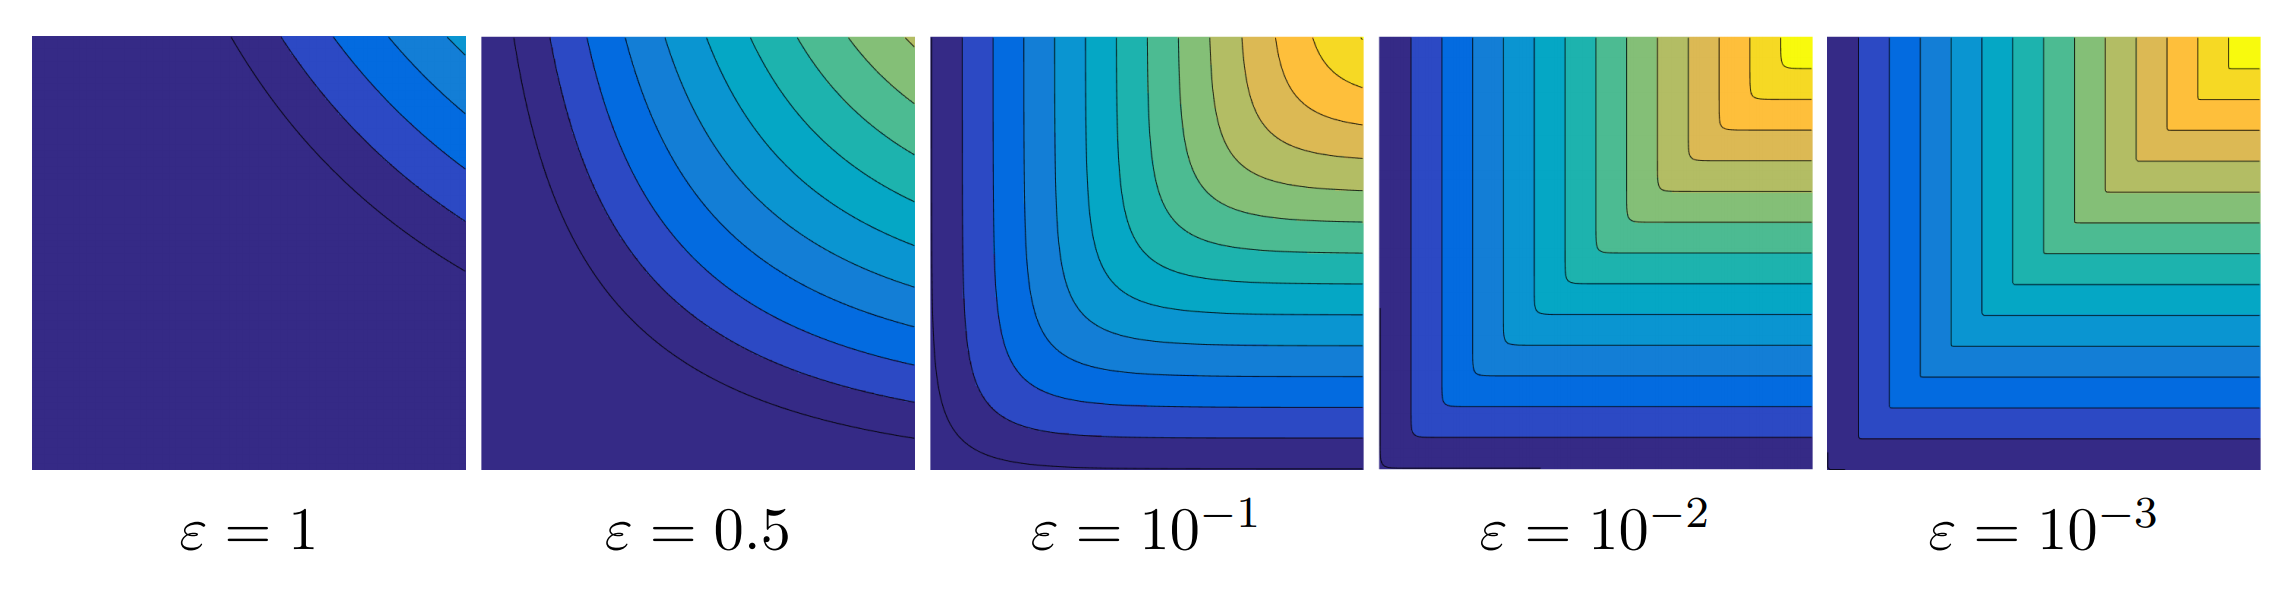
\includegraphics[width=0.9\linewidth]{img/min_eps}
  \label{fig:ot}
  \caption{Soft-minimum}
\end{figure}

Using this notation,

\begin{equation}
  \begin{array}{l}
    {\left(\mathbf{f}^{(\ell+1)}\right)_{i}=\min _{\varepsilon}\left(\mathbf{C}_{i j}-\mathbf{g}_{j}^{(\ell)}\right)_{j}+\varepsilon \log \mathbf{\mu}_{i}} \\
    {\left(\mathbf{g}^{(\ell+1)}\right)_{j}=\min _{\varepsilon}\left(\mathbf{C}_{i j}-\mathbf{f}_{i}^{(\ell)}\right)_{i}+\varepsilon \log \mathbf{\nu}_{j}}
    \end{array}
\end{equation}

To simplify notations, we introduce an operator that
takes a matrix as input and outputs now a column vector of the soft-minimum values
of its columns or rows. Namely, for any matrix $\mathbf{A} \in \mathbb{R}^{m \times n}$, we define

\begin{equation}
  \begin{array}{l}
    {\operatorname{Min}_{\varepsilon}^{\mathrm{row}}(\mathbf{A}) \stackrel{\text { def. }}{=}\left(\min _{\varepsilon}\left(\mathbf{\mu}_{i, j}\right)_{j}\right)_{i} \in \mathbb{R}^{m}} \\
    {\operatorname{Min}_{\varepsilon}^{\mathrm{col}}(\mathbf{A}) \stackrel{\mathrm{def}}{=}\left(\min _{\varepsilon}\left(\mathbf{\nu}_{i, j}\right)_{i}\right)_{j} \in \mathbb{R}^{n}}
    \end{array}
\end{equation}

Using this notation, Sinkhorn's iterates read

\begin{equation}
  \begin{array}{l}
    {\mathbf{f}^{(\ell+1)}=\operatorname{Min}_{\varepsilon}^{\mathrm{row}}\left(\mathbf{C}-\mathbf{1}_{m} \mathbf{g}^{(\ell)^{\mathrm{T}}}\right)+\varepsilon \log \mathbf{\mu}} \\
    {\mathbf{g}^{(\ell+1)}=\operatorname{Min}_{\varepsilon}^{\mathrm{col}}\left(\mathbf{C}-\mathbf{f}^{(\ell)} \mathbf{1}_{n}^{\mathrm{T}}\right)+\varepsilon \log \mathbf{\nu}}
    \end{array}
\end{equation}

While mathematically equivalent to the Sinkhorn
updates \ref{eq:sinkhorn}, iterations above suggest using the log-sum-exp stabilization
trick to avoid underflow for small values of $\epsilon$. Writing $\underline{z}=\min \mathbf{z}$, that trick suggests
evaluating $\min_{\varepsilon} z$ as

\begin{equation}
  \operatorname{min}_{\varepsilon} \mathbf{z}=\underline{z}-\varepsilon \log \sum e^{-\left(\mathbf{z}_{i}-\underline{Z}\right) / \varepsilon}
\end{equation}

Instead of substracting $\mathbf{z}$ to stabilize the log-domain iterations as above, one can actually substract the previously computed scalings. This leads to the stabilized iteration

\begin{equation}
  \begin{array}{l}
    {\mathbf{f}^{(\ell+1)}=\operatorname{Min}_{\varepsilon}^{\mathrm{row}}\left(\mathbf{S}\left(\mathbf{f}^{(\ell)}, \mathbf{g}^{(\ell)}\right)\right)-\mathbf{f}^{(\ell)}+\varepsilon \log (\mathbf{\mu})} \\
    {\mathbf{g}^{(\ell+1)}=\operatorname{Min}_{\varepsilon}^{\mathrm{col}}\left(\mathbf{S}\left(\mathbf{f}^{(\ell+1)}, \mathbf{g}^{(\ell)}\right)\right)-\mathbf{g}^{(\ell)}+\varepsilon \log (\mathbf{\nu})}
    \end{array}
\end{equation}

where we defined 

\begin{equation}
  \mathbf{S}(\mathbf{f}, \mathbf{g})=\left(\mathbf{C}_{i, j}-\mathbf{f}_{i}-\mathbf{g}_{j}\right)_{i, j}
\end{equation}

In contrast to the original iterations \ref{eq:sinkhorn}, these log-domain iterations
are stable for arbitrary $\epsilon$, because the quantity $\mathbf{S}(\mathbf{f}, \mathbf{g})$ stays bounded during the
iterations. The downside is that it requires nm computations of exp at each step. Computing a $\mathrm{Min}_{\varepsilon}^{\mathrm{row}}$ is typically substantially slower than matrix multiplications
and requires computing line by line soft-minima of matrices $\mathbf{S}$. There is therefore no
efficient way to parallelize the application of Sinkhorn maps for several marginals simultaneously. In Euclidean domains of small dimension, it is possible to develop efficient
multiscale solvers with a decaying $\epsilon$ strategy to significantly speed up the computation
using sparse grids.

\vspace{2ex}
    \begin{algorithm}[htbp]
        \SetAlgoNoLine
        \caption{Block Coordinate Ascent algorithm for regularized problem} 
        \KwIn{parameters $\mu$, $\nu$, $c$}
        \KwIn{epsilon $\epsilon$}
        Initialize variables $\mathbf{f}, \mathbf{g} = \boldsymbol{1}$\\
        Initialize  $\mathbf{K} = \exp^{-c/\epsilon}$\\
        \While{ stopping criterion not met } 
        {  
          Update $\mathbf{S}$: $\mathbf{S}(\mathbf{f}, \mathbf{g})=\left(\mathbf{C}_{i, j}-\mathbf{f}_{i}-\mathbf{g}_{j}\right)_{i, j}$\\
          Update $\mathbf{f}$: ${\mathbf{f}^{(\ell+1)}=\operatorname{Min}_{\varepsilon}^{\mathrm{row}}\left(\mathbf{S}\left(\mathbf{f}^{(\ell)}, \mathbf{g}^{(\ell)}\right)\right)-\mathbf{f}^{(\ell)}+\varepsilon \log (\mathbf{\mu})}$\\
          Update $\mathbf{S}$: $\mathbf{S}(\mathbf{f}, \mathbf{g})=\left(\mathbf{C}_{i, j}-\mathbf{f}_{i}-\mathbf{g}_{j}\right)_{i, j}$\\
          Update $\mathbf{g}$: ${\mathbf{g}^{(\ell+1)}=\operatorname{Min}_{\varepsilon}^{\mathrm{col}}\left(\mathbf{S}\left(\mathbf{f}^{(\ell+1)}, \mathbf{g}^{(\ell)}\right)\right)-\mathbf{g}^{(\ell)}+\varepsilon \log (\mathbf{\nu})}$\\
        }
        Calculate $\mathbf{u} = \exp(\mathbf{f}/\epsilon)$\\
        Calculate $\mathbf{v} = \exp(\mathbf{g}/\epsilon)$\\
        Calculate $\mathbf{P} = (\operatorname{diag}{\mathbf{u}}) \mathbf{K} (\operatorname{diag}{\mathbf{v}})$\\
    \end{algorithm}